\subsection{Gaussian Processes for Regression}
	For noisy measurements of (laboratory) values at certain time points it is difficult to fix
	what the best estimates of values between the time points or at future time points are.
	The assumption of an underlying linear function makes it easy to fit a straight line by least-squares method. But this is often a oversimplification of the problem. The model will provide poor predictions, if the relationship between  dependent and independent variable can not be approximated by a linear function.
	Even a polynomial regression models the changes of laboratory measurements  over time only unsatisfactorily with the problem of over-fitting
	
	Regression with \ac{GP} is a smarter method to model the relationship between successive measured values. 
	A Gaussian Process does not assume some specific model underlying the data but calculates the relationship between single data points.
	
	In principle are Gaussian Processes a generalization of multivariate Gaussian distributions toward infinite dimensionality.
	
	The $n$ observations of a (laboratory) data set $\pmb{y}=\{y_{1},y_{2}, \ldots ,y_{n}\}$ measured at the time points $\pmb{t}=\{t_{1},t_{2}, \ldots ,t_{n}\}$ could be imagined as a sample of a multivariate, n-variate Gaussian distribution:
	
	\begin{displaymath}
		\pmb{y} \sim N(\pmb{\mu},\Sigma)
	\end{displaymath}
	
	with the vector of means $\pmb{\mu}$ and the covariance matrix
	
	
	\begin{displaymath}
		\Sigma = cov(\pmb{y}) = K(\pmb{t},\pmb{t}) + \sigma^{2}_{n}I
	\end{displaymath}
	
	The elements of the covariance matrix $\Sigma$ are calculated by the covariance function k:
	
	\begin{displaymath}
		cov(y_{p},cov_{q}) = k(t_{p},t_{q}) + \sigma^{2}_{n} \delta_{pq}
	\end{displaymath}
	
	The covariance function \footnote{The terms covariance function, covariance kernel, kernel function and kernel are used interchangeably} is the key ingredient in using Gaussian processes \cite{Wilson_2013}. The selection of the covariance function depends on the assumptions about the form of the underlying  function that is modelled by the Gaussian process, e.g. smoothness, periodicity, etc.. The covariance function determines the similarity between observed values $y_{p}$ and $y_{q}$ at the time points $t_{p}$ and $t_{q}$. The closer the time points the greater is the similarity and the bigger is the value of the covariance function.  
	
	The de-facto default covariance function for \ac{GP} is the "Squared Exponential Kernel":
	
	\begin{displaymath}
		cov(y_{p},y_{q}) = k(t_{p},t_{q}) + \sigma^{2}_{n} \delta_{pq} = 
		e^{-\frac{(t_{p}-t_{q})^{2}}{2 \ell^{2}}} +
		\sigma^{2}_{n} \delta_{pq}
	\end{displaymath}
	
	This kernel is infinitely differentiable and can represent long range trends. The lengthscale $\ell$ determines how quickly the \ac{GP} varies with $t$ and the length of the alteration. It is not possible to explore more than $\ell$ units away from the measured data. 
	
	The density function of the n-variate Gaussian distribution, representing the Gaussian process is 
	
	\begin{displaymath}
	f(\pmb{y}|\pmb{\mu},\sigma^{2},\ell) = 
	\frac{1}{\sqrt{(2\pi)^{n}det(\Sigma)}}
	e^{- \frac{1}{2} (\pmb{y}-\pmb{\mu})^{T} \Sigma^{-1} (\pmb{y}-\pmb{\mu}) }
	\end{displaymath}
	
	
    \subsection{Estimation of parameters}
    The parameters $\pmb{\mu}$, $\sigma^{2}$ and $\ell$ of the covariance function has to be estimated from the observed data $\pmb{y}=\{y_{1},y_{2}, \ldots ,y_{n}\}$ measured at the time points $\pmb{t}=\{t_{1},t_{2}, \ldots ,t_{n}\}$.
    One possibility is \ac{ML} estimation \cite{wiki_maximum_likelihood}. This method estimates the parameters of the model by maximizing the probability of obtaining the observed data, the likelihood:
    
    \begin{displaymath}
    	L(\pmb{\mu},\ell,\sigma^{2}|\pmb{y}) = 
    	f(\pmb{y}|\pmb{\mu},\sigma^{2},\ell) = 
    	\frac{1}{\sqrt{(2\pi)^{n}det(\Sigma)}}
    	e^{- \frac{1}{2} (\pmb{y}-\pmb{\mu})^{T} \Sigma^{-1} (\pmb{y}-\pmb{\mu}) }
    \end{displaymath}       
    	
    To simplify the calculation logarithm of the likelihood, Log-Likelihood function, is used to estimate the maximum:
    
    \begin{align*}
    & LL(\pmb{\mu},\ell,\sigma^{2}|\pmb{y}) = \\
    & log(
    \frac{1}{\sqrt{(2\pi)^{n}det(\Sigma)}}
    e^{-\frac{1}{2}(\pmb{y}-\pmb{\mu})^{T} \Sigma^{-1} (\pmb{y}-\pmb{\mu})}) = \\
    & -\frac{1}{2} * n * log(2\pi) - \frac{1}{2} * log(det(\Sigma)) - \frac{1}{2} 
    (\pmb{y}-\pmb{\mu})^{T} \Sigma^{-1} (\pmb{y}-\pmb{\mu})
   \end{align*}
     
    The estimation of the parameters $\pmb{\mu}$, $\sigma^{2}$ and of the lengthscale $\ell$ means to find local maxima of the Log-Likelihood function. 
    
    For the example patient (fig. \ref{example_patient}) the estimated hyperparams are:
    \begin{itemize}
    	\item $\sigma^{2}$: 0.27
    	\item $\mu$: 2.87
    	\item $\ell$: 214  
    \end{itemize}
    
    So the covariance function is
    \begin{align}
    cov(y_{p},y_{q})=\exp^{\frac{(t_{p}-t_{q})^2}{91602.76}}+0.073*\delta_{pq}
    \end{align}
    
    \subsubsection{Accuracy of Maximum Likelihood Estimation - The Fisher information} 
	It is necessary to know how accurate the estimation of the parameters of the kernel is. This information is given by calculating the curvature of the likelihood function around the maxima. A sharp curvature around the maximum means a high certainty, while a flat course gives a signal for a quite uncertain estimation.
	A measure for the curvature of the score function is the variance of the score, called Fisher Information $I$ \cite{wiki_fisher_information}. 
	
	For the n-variate normal distribution of the \ac{GP} 
	\begin{displaymath}
		\pmb{y} \sim N(\pmb{\mu(\pmb{\theta})},\Sigma(\pmb{\theta}))
	\end{displaymath}
	
	is 
	
	\begin{displaymath}
		\pmb{\theta} = [\theta_{1} , \theta_{2} , \theta_{3}] = 
		[ \pmb{\mu} , \sigma^{2} , \ell ]
	\end{displaymath}
	
	the vector of the parameters of the distribution.
	
	The Elements $I_{m,n}$ for $1 \leq m,n \leq 3$ of the 3x3-\ac{FIM} is:
	
	\begin{displaymath}
		\mathcal{I}_{m,n} = 
		\frac{ \partial \pmb{\mu}^{T}}{\partial \theta_{m}}
		\Sigma^{-1}
		\frac{\partial \pmb{\mu}}{\partial \theta_{n}}
		+\frac{1}{2}tr(
		\Sigma^{-1}
		\frac{\partial \Sigma}{\partial \theta_{m}}
		\Sigma^{-1}
		\frac{\partial \Sigma}{\partial \theta_{n}}
		)
	\end{displaymath}
	
	and
	
	\begin{displaymath}
		\frac{\partial \pmb{\mu}}{\partial \theta_{m}} =
		[ 
		\frac{\partial \mu_{1}}{\partial \theta_{m}},
		\frac{\partial \mu_{2}}{\partial \theta_{m}},
		\ldots,
		\frac{\partial \mu_{N}}{\partial \theta_{m}}
		]
	\end{displaymath}
	
	\begin{displaymath}
	\frac{\partial \Sigma}{\partial \theta_{m}} =
		\begin{bmatrix}
			\frac{ \partial \Sigma_{1,1}}{\partial \theta_{m}} &
			\frac{ \partial \Sigma_{1,2}}{\partial \theta_{m}} &
			\ldots &
			\frac{ \partial \Sigma_{1,N}}{\partial \theta_{m}} \\
			\frac{ \partial \Sigma_{2,1}}{\partial \theta_{m}} &
			\frac{ \partial \Sigma_{2,2}}{\partial \theta_{m}} &
			\ldots &
			\frac{ \partial \Sigma_{2,N}}{\partial \theta_{m}} \\
			\vdots &
			\vdots &
			\ddots &
			\vdots \\
			\frac{ \partial \Sigma_{N,1}}{\partial \theta_{m}} &
			\frac{ \partial \Sigma_{N,2}}{\partial \theta_{m}} &
			\ldots &
			\frac{ \partial \Sigma_{N,N}}{\partial \theta_{m}} 
		\end{bmatrix}
	\end{displaymath}
	 
	The \ac{FIM} of estimated hyperparams of the example patient is   
	
	\begin{align}
		\bordermatrix{
	 			& \sigma^{2} & \mu & \ell \cr
	 		\sigma^{2} & 142.6 & 0.0 & -0.1 \cr
	 		\mu & 0.0 & 2.5 & 0.0 \cr
	 		\ell & -0.1 & 0.0 & 0.0 \cr
		}
	\end{align}
	
	\subsection{Estimation of distribution of \ac{GP} by bootstrapping}
	Using the results of estimating the hyperparams by maximum-likelihood and of calculating the connected \ac{FIM} it can be assumed that the estimated hyperparams are the realisation of a random sample from a empirical multivariate normal distribution. The n-dimensional mean of the distribution are the estimated hyperparams $\hat{\sigma_{2}}$,$\hat{\mu}$ and $\hat{\ell}$, the variance is the inverse of the \ac{FIM}:
	
	\begin{align}
		\pmb{\theta} = 
		\begin{bmatrix}
			\sigma^{2} \\
			\mu \\
			\ell
		\end{bmatrix}
		\sim N(
			\begin{bmatrix}
				\hat{\sigma_{2}} \\ \hat{\mu} \\ \hat{\ell}
			\end{bmatrix}
		,
		I^{-1}
		) 
	\end{align}   
	
	For the example patient the empiric normal distribution of the hyperparams is: 
	
	\begin{align}
	\pmb{\theta} = 
	\begin{bmatrix}
	\sigma^{2} \\
	\mu \\
	\ell
	\end{bmatrix}
	\sim N(
	\begin{bmatrix}
	0.27 \\ 2.87 \\ 30.57
	\end{bmatrix}
	,
	\begin{pmatrix}
		0.01 & 0.0 & 0.16 \\
		0.00 & 0.4 & 0.00 \\
		0.16 & 0.0 & 168.13 
	\end{pmatrix}
	) 
	\end{align}
	
	From this distribution a arbitrary number of random samples can be drawn. For each sample the \ac{GP} can be calculated and plotted. The overlaid plots then show the distribution of the \ac{GP}.

    \begin{figure}
    	\centering
    	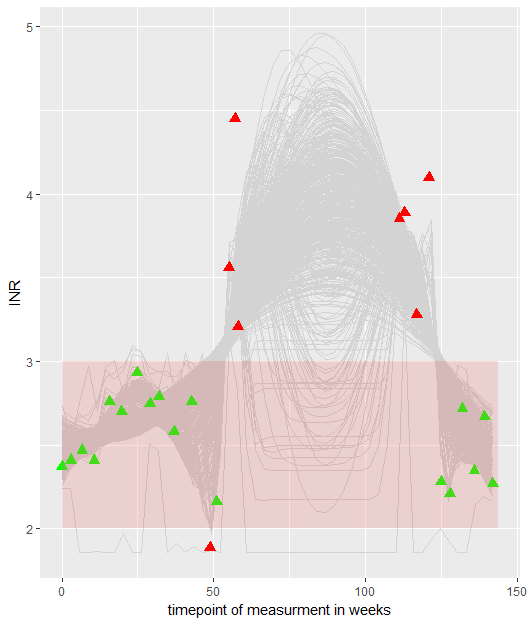
\includegraphics{./images/overlaid_gp_plots.png}
    	\label{overlaid_gp_plots}
    \end{figure}